\subsection{Разработка даталогической и физической моделей базы данных}
\label{sec:design:database}

На даталогическом уровне модель предметной области представляется в привязке к конкретной СУБД и описывает способ организации данных безотносительно их физического размещения.
Описывать модель можно с помощью специальных графических нотаций~\cite{kulikov_db_workbook}.

В программном средстве, описываемом данным дипломным проектом, предполагается использование встроенной в платформу \andro СУБД \sqlite.
Из преимуществ данной СУБД стоит отметить следующие особенности:
\begin{itemize}
    \item Самодостаточность –- базе данных \sqlite не требуется отдельный сервер для работы.
    Она встраивается прямо в приложение и требует только доступ к файлам.
    Поэтому её возможно использовать локально без соединения с удаленным сервером.
    \item Высокая производительность – \sqlite потребляет мало ресурсов операционной системы и в силу отсутствия необходимости передачи данных по сети позволяет выполнять значительно быстрее по сравнению со стандартными серверными СУБД.
\end{itemize}

Однако, данная СУБД достаточно сильно ограничена типам данных, что стоит учитывать при разработке физической модели базы данных программного средства.
Типы данных, поддерживаемые СУБД \sqlite~\cite{sqlite_types}:
\begin{itemize}
    \item \emph{NULL} -- пустое значение.
    \item \emph{INTEGER} -- знаковое целое число, сохраненное в 1, 2, 3, 4, 6 или 8 байтах вы зависимости от размера значения.
    \item \emph{REAL} -- число с плавающей точкой, сохраненное в 8 байтах по стандарту IEEE-754~\cite{ieee_754}.
    \item \emph{TEXT} -- строковое значение, сохраненное в кодировке UTF-8.
    \item \emph{BLOB} -- бинарные данные, сохраненные точно в том же виде.
\end{itemize}

В проектируемом программном средстве существует необходимость хранить данные некоторых типов, которые не поддерживаются данной СУБД, среди них:
\begin{itemize}
    \item временные значения;
    \item логические значения.
\end{itemize}

С учётом ограничений, временные значения предполагается хранить в текстовом виде с форматом записи по стандарту ISO~8601~\cite{iso_8601}.
Логические значения легко сохранять в качестве целочисленных значений 1 (Истина) и 0 (Ложь).

Также существует необходимость хранения нецелых денежных сумм, так как некоторые валюты могут состоять из дробных частей.
Для избежания погрешности в арифметических операциях с числами с плавающей точкой, предполагается хранение данных денежных сумм в текстовом виде с округлением до двух знаков после запятой.

Физическая модель базы данных представлена на рисунке~\ref{fig:design:database:model}.

Рассмотрим подробнее некоторые особенности физической модели базы данных:
\begin{enumerate}
    \item Каждая сущность представлена своей таблицей.
    \item Все таблицы сущностей имеют поля, предназначенные для хранения глобального идентификатора (external\_id).
    По умолчанию имеют эти поля имеют значение NULL, потому, что новые данные, созданные локально, не могут иметь глобального идентификатора без успешной синхронизации.
    \item Журналы изменений, описанные в подразделе~\ref{sec:design:sync} для каждой сущности представлены в виде отдельных таблиц, которые содержат в себе все поля, что и таблицы сущностей, но с некоторыми дополнительными атрибутами:
    \begin{enumerate}
        \item Action\_id представляет собой уникальный идентификатор записи в журнале.
        \item Action\_type указывает на то, какой тип операции был произведен над сущностью.
        Предполагается, что поле может содержать одно из значений <<INSERT>>, <<UPDATE>> и <<DELETE>>.
        \item Action\_timestamp отображает время совершения операции для последующего определения приоритета в конфликтных ситуациях.
    \end{enumerate}
    \item Параметры отображения сущности <<Валюта>> в физической модели базы данных представлены двумя атрибутами:
    \begin{enumerate}
        \item Symbol -- строковое значение, содержащее в себе знак валюты или общепринятую подпись денежных значений в данной валюте.
        Например, для валюты <<Белорусский рубль>> данное поле будет содержать значение <<руб.>>.
        \item Is\_prefix указывает на то, каким образом должна производиться запись подписи валюты и самого значения.
        При значении is\_prefix равным единице подпись валюты располагается до значения суммы.
    \end{enumerate}
    \item Атрибут <<Сумма перевода>> сущности <<Перевод между счетами>> в физической модели представлен двумя атрибутами, отображающими суммы переводов счёта-отправителя и счёта-получателя соответственно.
    Разделение данного атрибута необходимо для поддержки множественных валют, так как эти суммы могут не совпадать.
\end{enumerate}

\begin{figure}[H]
    \centering
    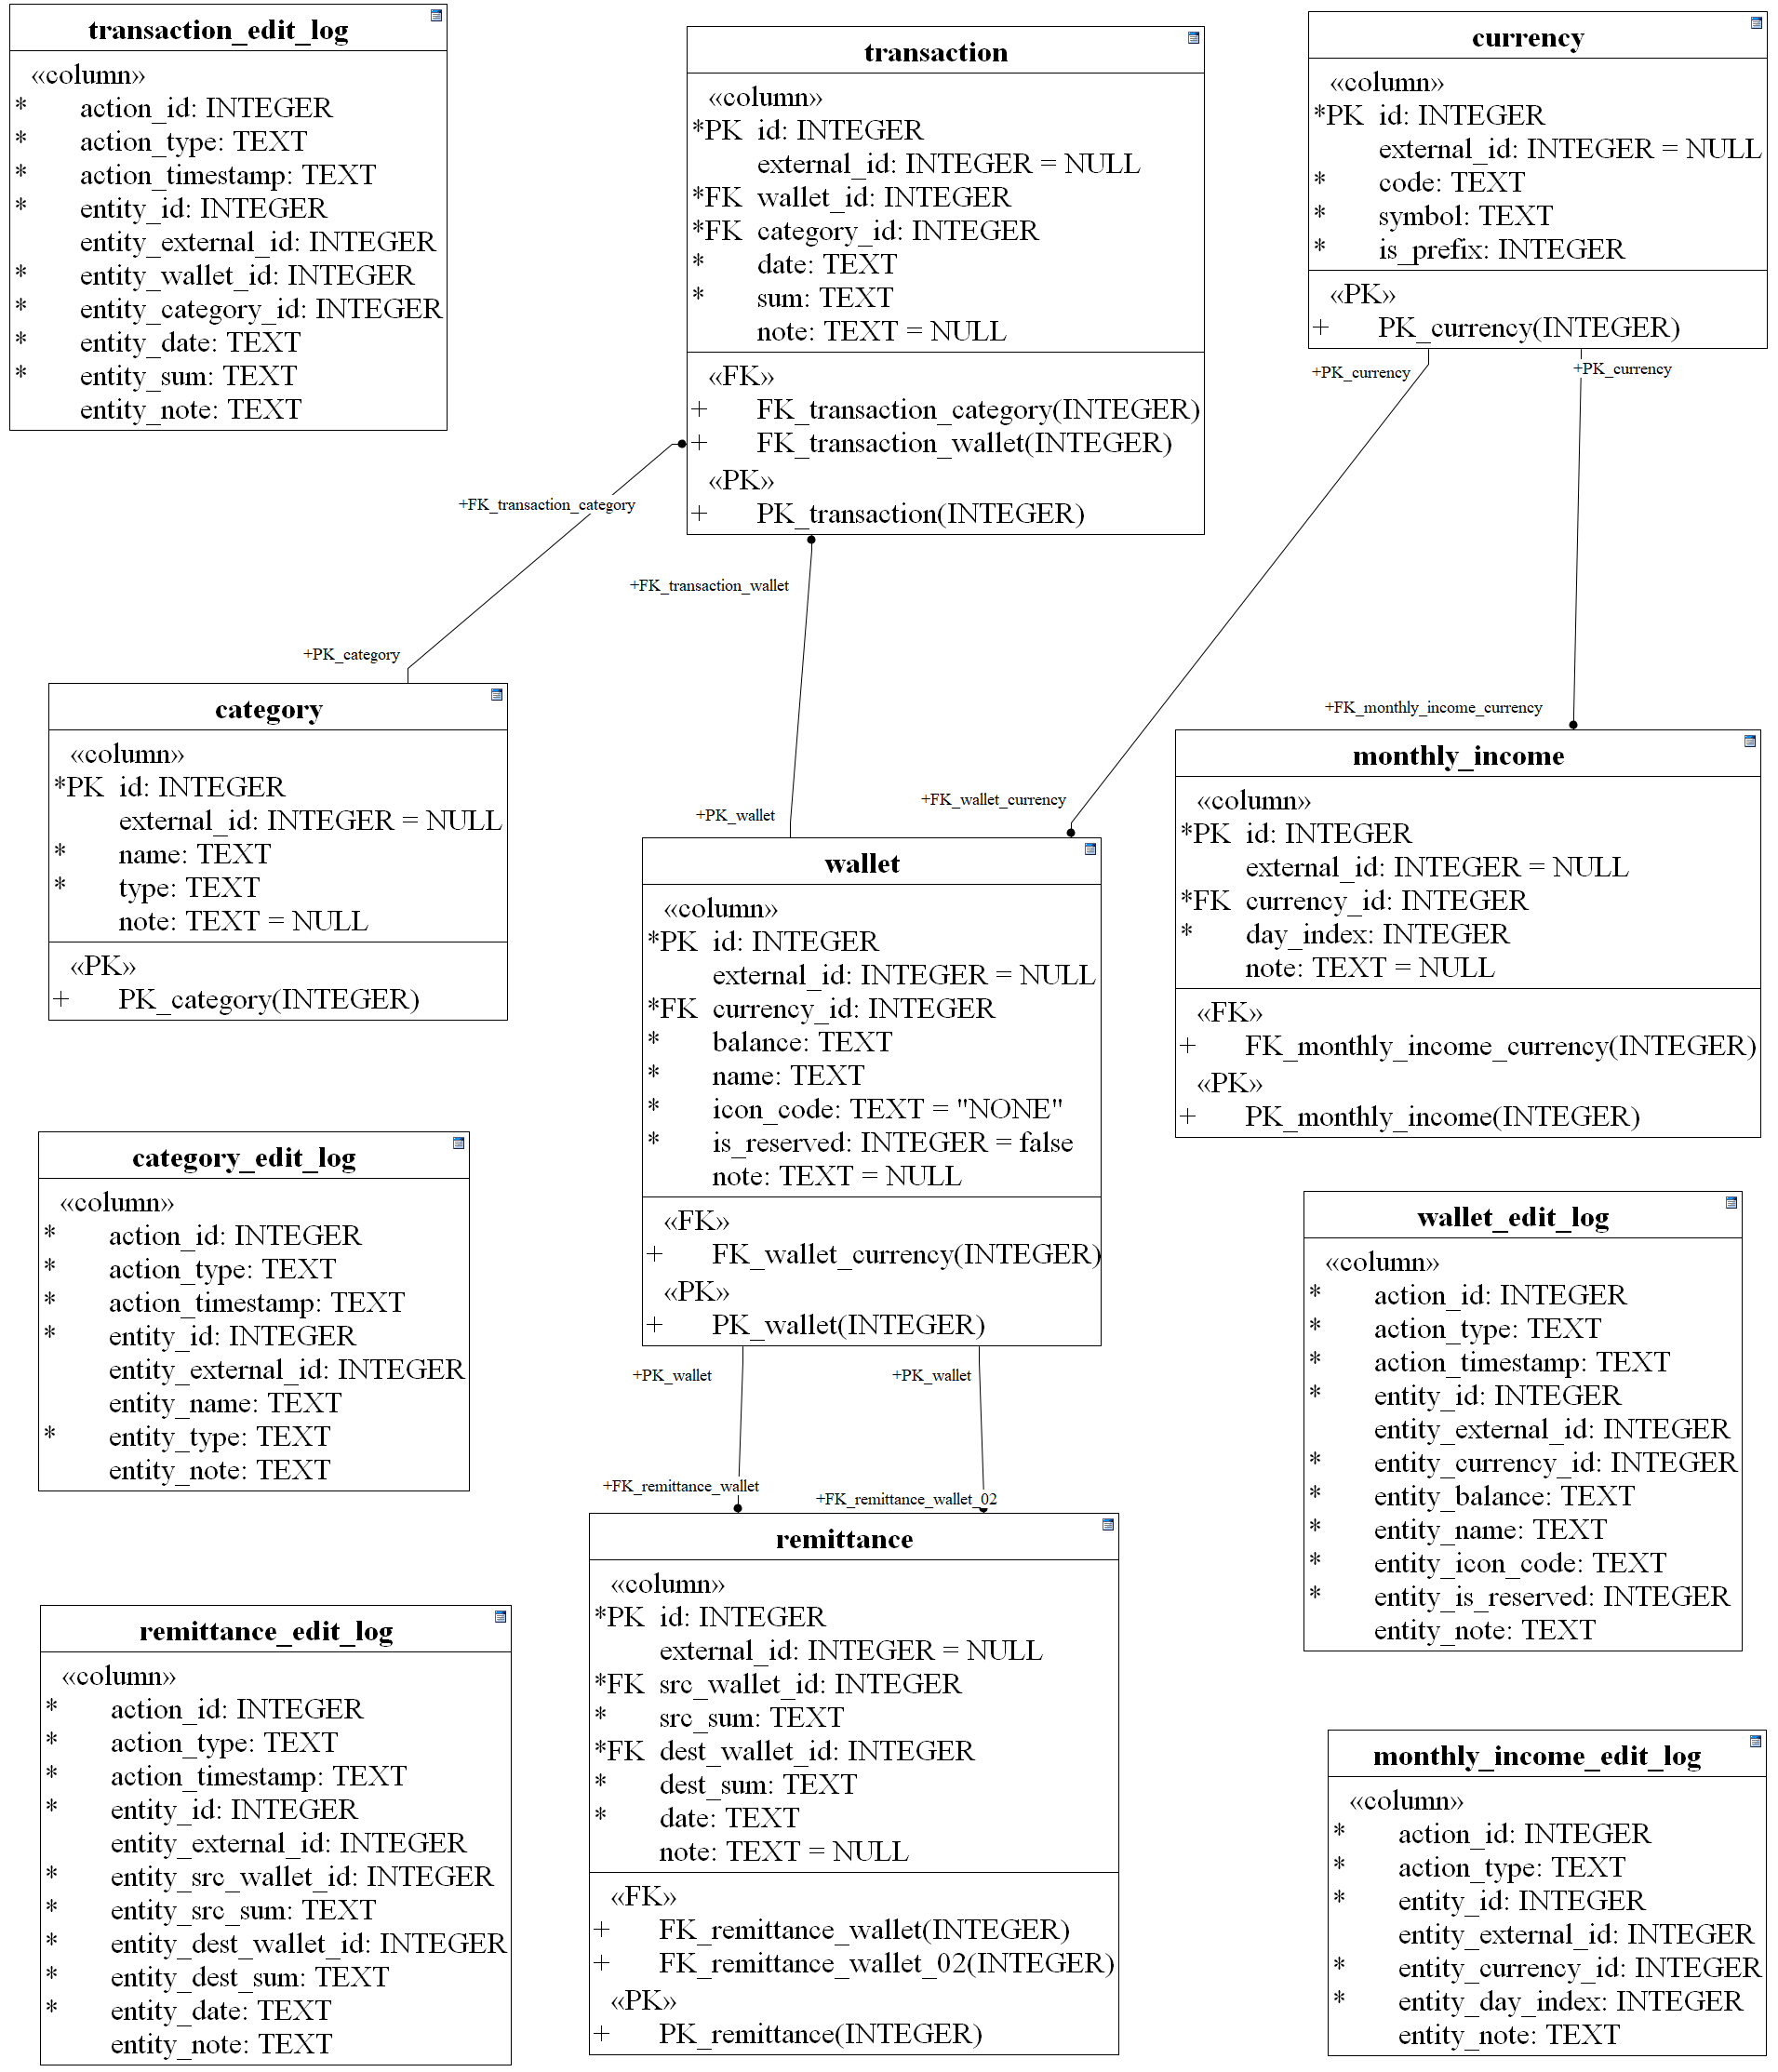
\includegraphics[scale=0.38]{3_3_physical_model.png}
    \caption{Физическая модель базы данных ПС}
    \setlength\intextsep{2pt}
    \label{fig:design:database:model}
\end{figure}

Регистрация операций с сущностями в таблицах журналов изменений можно реализовать при помощи встроенных в СУБД \sqlite при помощи триггеров -- хранимых процедур особого типа, исполнение которых обусловлено действием по модификации данных над определённой таблицей базы данных.
Таким образом, при проведении операции с какой-либо таблицей сущности, изменения будут автоматически записываться в соответствующую таблицу журнала изменений.
